\documentclass [11pt, proquest] {uwthesis}[2020/02/24]
\usepackage{graphicx}
\graphicspath{ {./images/} }

\setcounter{tocdepth}{1}  % Print the chapter and sections to the toc

\let\mffont=\sf

\begin{document}

\prelimpages

\Title{Securing WireGuard private keys with a hardware token\\}
\Author{Peter Van Eenoo}
\Year{2022}
\Program{Computer Science and Engineering}

\Chair{Brent Lagesse}{Dr.}{Computing \& Software Systems}
\Signature{William Erdly}
\Signature{Yang Peng}

\copyrightpage

\titlepage  


\setcounter{page}{-1}
\abstract{

The WireGuard VPN has had a successful mainstream adoption, as evidenced by its recent inclusion in many 
open-source operating systems\cite{donenfeld_wireguard_nodate} as well as a recent native Windows kernel module\cite{noauthor_wireguard-nt_nodate}. 
WireGuard does not use x509 certificates or the traditional PKI infrastructure. Key management is intentionally left up to the users which can causes a problem because the client key is not easily associated with a user or system and cannot be revoked, except by removing the client’s public key from all servers.
The client and server’s public key consist of a single 256-bit public key based on Curve25519 
which must be pre-shared with the server and client respectively before a successful handshake can be made. 
On a Linux laptop for example, the private key is held in a plain-text file along with the server’s public key and IP address. 
Securing this file is left up to the user and it would be an easy target for malware or a malicious party to steal.
The WireGuard protocol implements perfect forward secrecy, meaning loss of a private key still won’t allow past conversations to be decrypted. 
However, secure key management is still very important because loss of the client’s private key would result in two major vulnerabilities. 
First, it would allow an attacker to connect the target VPN undetected, masquerading as a legitimate client for any system where the private key is trusted. 
Secondly, it would enable the attacker to perform a persistent DoS attack against the client’s connection to the server.
If malware were programmed to look for WireGuard configuration files, collecting the keys and connecting to remote systems would be trivial 
for attackers and hard to detect for system administrators.



%\footnote{See Appendix A to obtain the source to this
% thesis and the class file.}
}

%
% ----- contents & etc.
%
\tableofcontents
\listoffigures

\chapter*{Glossary}      % starred form omits the `chapter x'
\addcontentsline{toc}{chapter}{Glossary}
\thispagestyle{plain}

\begin{glossary}

\item[Security Key]
A device that securely stores cryptographic keys and restrict access through a limited interface. 
Nitrokey Start\cite{noauthor_nitrokey_nodate} or the more common YubiKey\cite{noauthor_discover_nodate}\cite{noauthor_u2f_nodate-1}, are a class of security keys that implement a user-controlled 
cryptographic authenticator which are resistant to malware and phishing attacks and are essentially a hardware security module (HSM). 
These devices typically connect to a computer or smartphone via USB or NFC

\item[WireGuard]

a VPN technology proposed in 2017 that operates at the network layer, which aims to replace popular TLS-based VPNs like OpenVPN and IPsec.
WireGuard has been described as “crypto-opinionated”, meaning the WireGuard protocol supports only one cryptographic primitive for each cryptographic requirement.
There is no support for negotiation of cryptographic parameters. For example, WireGuard only supports ChaCha20 for symmetric 
encryption\cite{donenfeld_wireguard_2017} of data and Curve25519 key pairs for client authentication.

\item[Curve25519]
digital signature operations are referred to as Ed25519. Key-signing operations are referred to as x25519. 
This distinction is important because WireGuard uses only x25519 operations for Elliptic-curve Diffie–Hellman (ECDH) key exchange, 
when generating the symmetric cipher key.


\end{glossary}

\textpages

\chapter {Introduction}
WireGuard is a new implementation of an open-source Virtual Private Network (VPN) introduced in 2018.

\section {Background}
Background is important to have for big papers
Provide background here

\section {Contributions}
The Curve25519 algorithm is being used in an increasing number of open-source and commercial products\cite{noauthor_things_nodate-1} from SSH to Signal, however hardware support in popular 
security keys is currently almost non-existent. YubiKey is currently the most popular security key manufacturer however all of their current products 
lack support for x255191. I hope my project will encourage more manufactures to add support for x25519 in their security keys.


\section {Methodology}
In order to evaluate what I have done, I will do XYZ and present my findings

\chapter {Creating the system}

\section {Starting}
When I started on the project in full, after receiving the go-ahead in August and fall quarter began, I didn't know where to begin but I knew I had start with something that would demonstrate my ability to get this project going.
I figured that interfacing with the NitroKey would be the first order of business. If the key is held on that device, than I should be able to create one and sign some data with it. I initially chose the nitrokey start because it's product page said it supported X25519\cite{noauthor_nitrokey_nodate} which is the ECDH key derivation process. After a few frustrating days I couldn't figure out how to even generate or put a curve25519 key on the nitrokey start, nor had I found any software that interfaced with a nitrokey start for performing x25519 operations. What I did discover after pouring over NitroKey's documentation was that they recommended using a program called OpenSC to work with the Nitrokey but that only a program called GnuPG was capable of telling the Nitrokey to generate a curve25519 key. One important detail was that GnuPG could generate the keys but didn't support key derivation so I couldn't use it to do x25519.

It was a frustrating start to my project, I couldn't' even start on modifying WireGuard to use the NitroKey if I couldn't create a proof-of-concept program that would perform the key derivation operation on the Nitrokey itself.
\section {OpenSC}
Key derivation for ECDH, called X25519 in my specific case, requires access to user Bob's private key and access to user Alice's public key. The operation will generate a new 'shared' key that is identical for both parties when the keys are flipped and you use Alice's private key and Bob's public key.
After researching the OpenSC tool support forums, I was able to find the command string that should have allowed me to perform the operation on the key, however it refused to read my public key. I found out that while NitroKey said OpenSC was the best tool to use with the nitrokey, OpenSC didn't support reading curve25519 keys! Later I found that there was a single test that was written in OpenSC which used the PKCS11 interface to generate and verify a shared-secret on the hardware device but this functionality wasn't exposed to users in any way. Technically, OpenSC could be used to test that X25519 operations worked on a hardware device but with no user control over the process. This realization set the stage for the rest of the project: technically the functionality is there but no-one has a practical implementation yet, that I could find.

This gave me enough information to start looking into curve25519 support in OpenSSL. Curve 25519 support was a relatively recent addition in version 1.1 of the program\cite{noauthor_support_nodate}.
After digging through the OpenSC tool and reading the OpenSSL function documentation, I was able to upgrade how OpenSC read public-keys during key derivation and expand it's functionality to support X25519 and get the previous command working.
Once I had OpenSC working to perform X25519 on the key, I wrote a test that would perform the operation on the security key and also perform the operation as the other party but in software-only mode, using OpenSSL. At the end the test would verify the output was the same for both operations, thereby confirming the operations was producing valid output.
\subsection {my subsection}
Minor points

\section{pkclient}
Once I had X25519 working on the security key, the next logical step was to integrate this functionality into a program that could handle the various states that the hardware-key system could be in, abstracting the functionality enough so that it could be easily integrated into WireGuard.  I attempted to modify and build a kernel module but I got no where working by myself for a few days. Working with OpenSC felt like enough C code for the meantime and I needed to make progress on my project. There is a Go language (Golang) version of WireGuard that appeared easy to read and it's portable, meaning it works on many different versions. I decided to focus my efforts into modifying that version of WireGuard because it would be the fastest way to demonstrate the functionality of my program.
The Go programming language has good support for modules which allows programs to easily expand their functionality by importing other code modules. After some more research I realized I could create a Golang module that handled the security-key interface and exposed it to a calling program. 
Pkclient can handle logging into the security-key, prompting the caller for the pin, if the pin is not saved in the configuration file (optional), finding the appropriate x25519-key on the security-key and finally pkclient can handle key derivation requests and returning the derived-key back to the caller.

\section{configuration}
WireGuard configuration on the command-line is handled via a separate program called wireguard-tools \cite{noauthor_wireguard-tools_2022}. This program handles parsing a plain-text configuration file and turns the configuration directives into API calls to the separately running WireGuard daemon which configures the virtual-interface. I wanted my program to conform as closely as possible to the WireGuard reference implementation, so I made modifications to the wireguard-tools program and added support for an 'HSM' line in the plain-text configuration file. 
\begin{figure}[h]
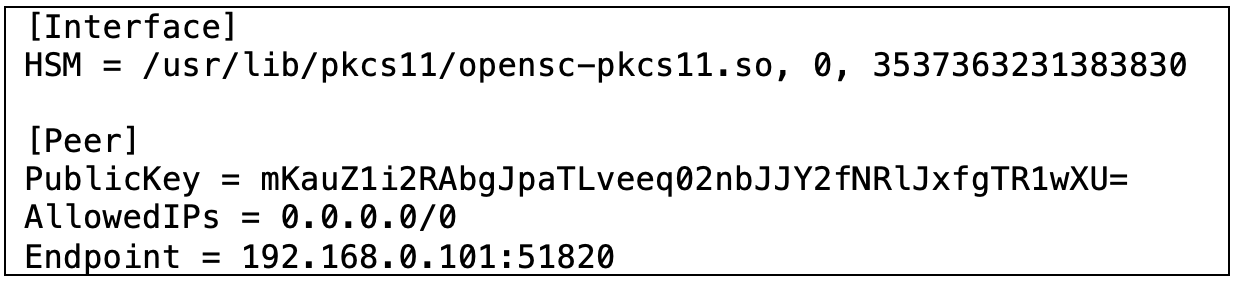
\includegraphics[width=8cm]{paper/images/wg_conf_hsm.png}
\end{figure}
This modification removes the requirement for defining and storing the private-key in the plain-text file and instead, tells the program what PKCS#11 library path, the slot on the key and optionally, the pin required to access the slot.

The inner-workings of the PKCS\#11 interface are out of scope for this document, however it suffices to say that for interfacing with a security-key, PKCS\#11 requires a slot ID and a pin-number for that slot, before the calling program an request operations on objects held on the slot. The PKCS\#11 interface will inform the caller if they successfully logged into the slot and if the requested operation suceeded or not.

Security is a balancing act between overall system security and user-convenience. Making a system more secure can often come at expense of user-convenience. Pkclient was written to give the user a choice in saving the pin-number in the configuration or omit it entirely. When the pin is omitted and the configuration file is read to wireguard-hsm, the program will prompt the user for the pin before the virtual interface is fully configured. If pkclient doesn't have the pin number for the given slot, it cannot be sure the key is configured properly. Saving the security-key pin-number in the configuration file reduces the security of our system a little but a given-user's threat-model may not require that the pin remains a secret since the user has physical control over the token. This case is called in out THREAT_MODEL_REFERENCE


PKCS\#11 is the standard interface for interacting with hardware security modules, logging into them and requesting operations, getting output back, all while the keys stay protected on the device.
My next step for incremental building was to create an interface program that could login to a hardware key, find a curve25519 key and perform key derivation operations.

\chapter {threat-model}
WireGuard has been
\section{improving WG}
Our primary threat-model guards against malware that runs on user's computer and gains access to the plain-text configuration file for WireGuard, leaking the private key which gives the bad-actors the ability to connect to the configured wireguard-peers undetected, as the legitimate user.

\chapter {Data1}

\chapter {Discussion of Results}
\section {Introduction}
I will discuss the limitations of my project as well as the technical hurdles that I faced while implementing and evaluating my project.

\section {Limitations}
I had initially hoped that my project could include mobile operating systems such as a smart phone. Users can easily use security keys
with mobile operating systems but due to technical requirements of the WireGuard protocol, a user would have to leave their security key connected
to their smartphone permanently, which could only be accomplishing using duct-tape for NFC devices or leaving a USB device inserted into their USB port, which 
seems like a hazard for the device. This always-connected requirement exists because the WireGuard protocol performs a re-key operation between peers at a default 120 seconds 
or after 2\textsuperscript{60} messages are exchanged. I could require users to modify their WireGuard server and client to default to a much longer 
timeout for re-key but this seems like a burdensome approach and it's not possible in all situations for the client to modify server settings.

More issues discussed here 


\chapter {CONCLUSION AND FUTURE WORK}



\section {Future Work}
There are several areas where I would like to improve WireGuard-HSM that have been identified over the course of implementing the program.

\subsection{Pin Handling}
 If a user chooses not a save the security-key pin in the wireguard-hsm configuration file, then the program must prompt user for the pin. Currently this prompt is very simple and given on the command-line when the user runs WireGuard-HSM. This prompt is easy to miss and wouldn't work very well if WireGuard-HSM was implemented as a kernel module. A better approach would be to have the prompt implemented as a system-dialog window, that appears over any existing windows, making very simple for the user to omit the pin and only enter it when using WireGuard-HSM.

\bibliographystyle{plain}
\bibliography{references}
\end{document}
